\begingroup
\newcommand{\GerlingSeconds}[2]{#1\makebox[.42em][c]{,\makebox[0pt][r]{\textsuperscript{s}}}#2}
\begin{center}
\textsc{Gauss} to \textsc{Gerling}.\quad Göttingen, 11~August 1823.
\end{center}

\par\noindent\hspace*{\parindent}\mbox{.\ .\ .\ .\ .\ .\quad Your} wording, \textls[120]{if} I wished to sight from the Brocken on heliotrope light and did not prefer the little house, etc., seems to point to some misunderstanding of the reasons why I might go up the Brocken a second time.
Determining the direction to the Inselsberg precisely is indeed a principal objective, and there can be no question of sighting on the house at this distance, given how low and irregular it is.
Heliotrope light from the Inselsberg to the Brocken is therefore naturally the conditio sine qua non for my going there.
\par\noindent\hspace*{\parindent}This one reason alone, however, would still not justify my visiting again.
My 1821 measurements of the angles to my
\par\clearpage
\noindent\null\hfill{\small\textbf{ON THE HANOVER TRIANGULATION.}}\hfill\makebox[0pt][r]{\fontsize{13}{16}\selectfont 383}\par\medskip
\noindent own principal points had come out too scanty and not quite worthy of the whole enterprise, with the itinerant heliotrope and the unfavourable weather. I therefore wanted to repeat them by stationing heliotropes simultaneously at the points, and later to return once more to the Hohehagen and the Hils as well.
\par\noindent\hspace*{\parindent}Much as I would be delighted to send light for light from the Brocken and the Hohehagen to the Inselsberg, I am unable to spare you one of my heliotropes for this. If I had to cover the Hohehagen, the Hils, and perhaps Lichtenberg with a single itinerant heliotrope, I would get no further than in 1821.
\par\noindent\hspace*{\parindent}I can see several ways of getting around this:
\par\noindent\hspace*{\parindent}1) If you arrive at the Inselsberg and I at the Brocken at the same time and we send light to each other, with my assistant under orders to send you light from the Hohehagen from time to time and yours to send me light from the Meisner, then, with the benefit of the kind of weather often seen at the beginning of September, I can finish on the Brocken in a few days, perhaps in three. I can leave the assistant there with the heliotrope (he will continually send you light at the Inselsberg, as will the one on the Hohehagen), hurry to the Hohehagen, signal my arrival to you, and complete the work there relating to the Inselsberg in another few days (weather permitting). You can then dispose of your Inselsberg heliotrope as you please.
You will then receive light from the Hohehagen \textls[120]{continuously} for as long as I am there and, if you still need it, now and then once I am on the Hils.
\par\noindent\hspace*{\parindent}With regard to this plan, everything will therefore depend on whether you consider the connection with the Brocken and the Hanoverian triangles important enough to postpone stationing heliotropes on the Knill and the Milseburg until that plan has been carried out.
\par\noindent\hspace*{\parindent}2) Although I would prefer the course indicated above, since it establishes the connection between the measurements most completely, you could \textls[120]{if necessary} release the Inselsberg heliotrope earlier, as soon as I leave the Brocken, which can be made known by signals.
For the Hohehagen–Inselsberg direction, I would then have to be content with what I obtained in 1821 using \textsc{Encke}'s helio-
\par\clearpage
\noindent\makebox[0pt][l]{\fontsize{13}{16}\selectfont 384}\hfill{\small\textbf{CORRESPONDENCE WITH GERLING.}}\hfill\null\par\medskip
\noindent trope.
It goes without saying that you would have to determine the position of the new stone and the heliotrope site relative to the \textls[120]{house} as precisely as possible.
I repeat, however, that it would be better if I could obtain the angle from the Inselsberg to the Brocken directly on the Hohehagen.
\par\noindent\hspace*{\parindent}3) The best course of all would probably be for you to obtain a third heliotrope at once.
The gains in accuracy and time that you would derive from it in future would surely more than outweigh the small expense.
This would be all the easier now because \textsc{Rumpf} happens to have a new heliotrope ready.
He made one for \textsc{Schumacher} (and has already sent it) and on that occasion made two at once, since, as he says, it is easier to work that way.
The second is therefore still available at present, though there is no doubt that he will easily find another opportunity to sell it.
(I have already received several enquiries from abroad.)
I have asked Mr.~\textsc{Rumpf} to make this heliotrope completely ready for shipment and to refrain from giving it to anyone else until you have made known your decision about it.
If you are interested in it, perhaps the safest and quickest course would be to have it sent to the Meisner or have it picked up.
\par\noindent\hspace*{\parindent}4) I could also set out for the Brocken somewhat earlier than you set out for the Inselsberg. You would therefore have to try to obtain the direction to the Inselsberg from the Milseburg before all others, so that, from the day to be agreed on when I arrive on the Brocken, your assistant sends me light from the Inselsberg to the Brocken continuously.
You would then need to keep your heliotrope on the Inselsberg for a shorter time after your own arrival.
\par\noindent\hspace*{\parindent}But if all this should prove incompatible with your plans, I would have to give up the entire expedition, at least for this year (in which case I ask you to let me know as soon as possible, so that my assistants and I can make our arrangements accordingly). I also do not know whether I would be able to make arrangements next year to the same extent as I can this time.
This time, that is, I offer to leave the starting time entirely up to you.
Just tell me precisely the \textls[120]{day} from which you will reliably send me light from the Inselsberg to the Brocken.
I shall definitely be there on that day, and in cases 1,
\par\clearpage
\noindent\null\hfill{\small\textbf{ON THE HANOVER TRIANGULATION.}}\hfill\makebox[0pt][r]{\fontsize{13}{16}\selectfont 385}\par\medskip
\noindent 2, 3 I shall also send you heliotrope light at once. In case 4, I shall do so as soon as your light gives the single attention signal, timed by ordinary clock beats of \GerlingSeconds{0}{4}, namely:
\par\smallskip
{\centering
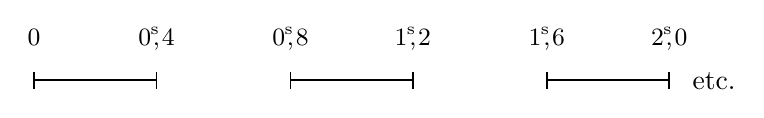
\begin{tikzpicture}[x=.0074cm,y=.0074cm,inner sep=0pt,outer sep=0pt,line width=.65pt]
\node[font=\small,anchor=base] at (0,60) {0};
\node[font=\small,anchor=base] at (210,60) {\GerlingSeconds{0}{4}};
\node[font=\small,anchor=base] at (440,60) {\GerlingSeconds{0}{8}};
\node[font=\small,anchor=base] at (650,60) {\GerlingSeconds{1}{2}};
\node[font=\small,anchor=base] at (880,60) {\GerlingSeconds{1}{6}};
\node[font=\small,anchor=base] at (1090,60) {\GerlingSeconds{2}{0}};
\draw (0,0)--(210,0) (0,-15)--(0,15) (210,-15)--(210,15);
\draw (440,0)--(650,0) (440,-15)--(440,15) (650,-15)--(650,15);
\draw (880,0)--(1090,0) (880,-15)--(880,15) (1090,-15)--(1090,15);
\node[anchor=base west] at (1130,-15) {etc.};
\end{tikzpicture}\par}
\par\noindent\hspace*{\parindent}I should point out, however, that the mirror must always be covered quite completely and should remain covered somewhat longer than it is open. I mean as follows:
\par\smallskip
{\centering
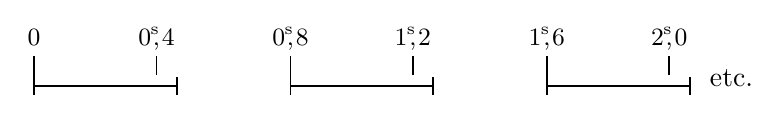
\begin{tikzpicture}[x=.0074cm,y=.0074cm,inner sep=0pt,outer sep=0pt,line width=.65pt]
\node[font=\small,anchor=base] at (0,70) {0};
\node[font=\small,anchor=base] at (210,70) {\GerlingSeconds{0}{4}};
\node[font=\small,anchor=base] at (440,70) {\GerlingSeconds{0}{8}};
\node[font=\small,anchor=base] at (650,70) {\GerlingSeconds{1}{2}};
\node[font=\small,anchor=base] at (880,70) {\GerlingSeconds{1}{6}};
\node[font=\small,anchor=base] at (1090,70) {\GerlingSeconds{2}{0}};
\draw (0,0)--(245,0) (0,-15)--(0,15) (245,-15)--(245,15);
\draw (440,0)--(685,0) (440,-15)--(440,15) (685,-15)--(685,15);
\draw (880,0)--(1125,0) (880,-15)--(880,15) (1125,-15)--(1125,15);
\draw (0,15)--(0,52) (210,20)--(210,52) (440,15)--(440,52) (650,20)--(650,52) (880,15)--(880,52) (1090,20)--(1090,52);
\node[anchor=base west] at (1160,-1) {etc.};
\end{tikzpicture}\par}
\par\noindent\hspace*{\parindent}I give other signals using numbers, for example the number 3, according to the following scheme:
\par\noindent\hspace*{\parindent}\textls[120]{I} give an indefinite number of attention signals until\\
\hspace*{\parindent}\textls[120]{you} reply with the same signals and continue until\\
\hspace*{\parindent}\textls[120]{I} stop, at which point you stop too and \textls[120]{pay attention}.
We may then wait about \(\frac{1}{4}\) minute.
I then give the signal itself as follows:
\par\smallskip
{\centering
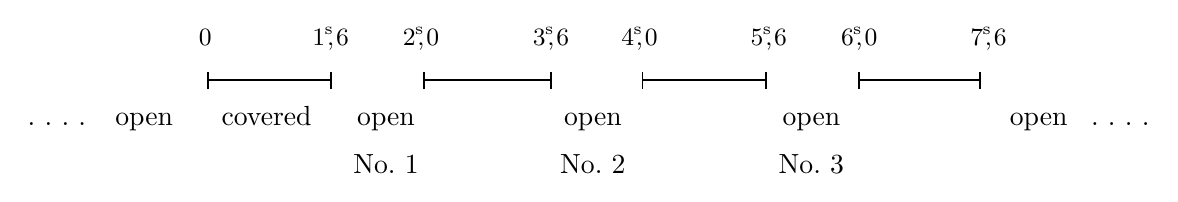
\begin{tikzpicture}[x=.0074cm,y=.0074cm,inner sep=0pt,outer sep=0pt,line width=.65pt]
\node[font=\small,anchor=base] at (360,60) {0};
\node[font=\small,anchor=base] at (575,60) {\GerlingSeconds{1}{6}};
\node[font=\small,anchor=base] at (730,60) {\GerlingSeconds{2}{0}};
\node[font=\small,anchor=base] at (953,60) {\GerlingSeconds{3}{6}};
\node[font=\small,anchor=base] at (1105,60) {\GerlingSeconds{4}{0}};
\node[font=\small,anchor=base] at (1327,60) {\GerlingSeconds{5}{6}};
\node[font=\small,anchor=base] at (1482,60) {\GerlingSeconds{6}{0}};
\node[font=\small,anchor=base] at (1704,60) {\GerlingSeconds{7}{6}};
\draw (365,0)--(575,0) (365,-15)--(365,15) (575,-15)--(575,15);
\draw (735,0)--(953,0) (735,-15)--(735,15) (953,-15)--(953,15);
\draw (1110,0)--(1322,0) (1110,-15)--(1110,15) (1322,-15)--(1322,15);
\draw (1482,0)--(1690,0) (1482,-15)--(1482,15) (1690,-15)--(1690,15);
\node[anchor=base west] at (55,-78) {\mbox{.\ .\ .\ .}};
\node[anchor=base] at (255,-78) {open};
\node[anchor=base] at (465,-78) {covered};
\node[anchor=base] at (670,-78) {open};
\node[anchor=base] at (1025,-78) {open};
\node[anchor=base] at (1400,-78) {open};
\node[anchor=base] at (1790,-78) {open};
\node[anchor=base west] at (1880,-78) {\mbox{.\ .\ .\ .}};
\node[anchor=base] at (670,-160) {No.~1};
\node[anchor=base] at (1025,-160) {No.~2};
\node[anchor=base] at (1400,-160) {No.~3};
\end{tikzpicture}\par}
\par\noindent\hspace*{\parindent}If the number is set \(=n\), the following alternate:
\par\smallskip
{\centering
\begin{tabular}{@{}r@{\quad}c@{\quad}l@{}}
 & \(n+1\) & times covered, for 4 beats,\\
with & \(n\) & times open, for 1 beat (in effect \(n\) flashes);
\end{tabular}\par}
\smallskip\noindent before and after, open, as specified, for a virtually indefinite time.
\par\noindent\hspace*{\parindent}You then repeat the same manoeuvre in reverse. Except when there has been a \textls[120]{long} interruption, however, you do so without waiting for my reply to your attention signal. Instead, after giving it about 10 to 20 times, you pause (open) for \(\frac{1}{4}\) minute and give the signal.
\par\noindent\hspace*{\parindent}Double signals, e.g.~\(3\,.\,3\), are announced by a double attention signal (\GerlingSeconds{0}{8} open and \GerlingSeconds{0}{8} covered). After the first number has been given, the mirror is left open for about 5 to \(10^{\mathrm{s}}\), and then the second number is given, thus:
\par\smallskip\noindent\hspace*{.035\linewidth}{\scriptsize IX.}\hfill{\normalsize49}\hspace*{.14\linewidth}\par
\clearpage
\noindent\makebox[0pt][l]{\fontsize{13}{16}\selectfont 386}\hfill{\small\textbf{CORRESPONDENCE WITH GERLING.}}\hfill\null\par\medskip
{\centering
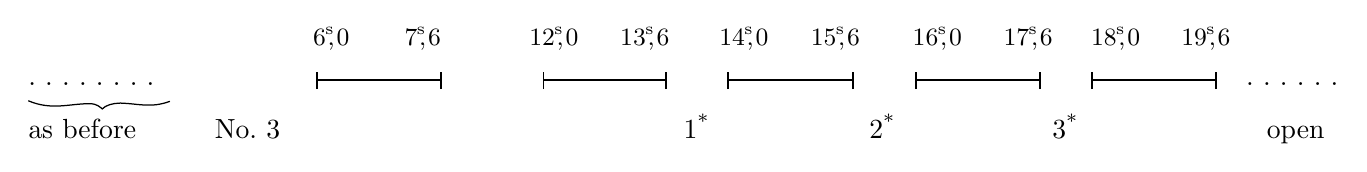
\begin{tikzpicture}[x=.0074cm,y=.0074cm,inner sep=0pt,outer sep=0pt,line width=.65pt]
\node[font=\small,anchor=base] at (540,60) {\GerlingSeconds{6}{0}};
\node[font=\small,anchor=base] at (697,60) {\GerlingSeconds{7}{6}};
\node[font=\small,anchor=base] at (922,60) {\GerlingSeconds{12}{0}};
\node[font=\small,anchor=base] at (1078,60) {\GerlingSeconds{13}{6}};
\node[font=\small,anchor=base] at (1248,60) {\GerlingSeconds{14}{0}};
\node[font=\small,anchor=base] at (1405,60) {\GerlingSeconds{15}{6}};
\node[font=\small,anchor=base] at (1580,60) {\GerlingSeconds{16}{0}};
\node[font=\small,anchor=base] at (1736,60) {\GerlingSeconds{17}{6}};
\node[font=\small,anchor=base] at (1886,60) {\GerlingSeconds{18}{0}};
\node[font=\small,anchor=base] at (2041,60) {\GerlingSeconds{19}{6}};
\draw (516,0)--(728,0) (516,-15)--(516,15) (728,-15)--(728,15);
\draw (904,0)--(1115,0) (904,-15)--(904,15) (1115,-15)--(1115,15);
\draw (1221,0)--(1435,0) (1221,-15)--(1221,15) (1435,-15)--(1435,15);
\draw (1544,0)--(1756,0) (1544,-15)--(1544,15) (1756,-15)--(1756,15);
\draw (1846,0)--(2058,0) (1846,-15)--(1846,15) (2058,-15)--(2058,15);
\node[anchor=base west] at (20,-8) {\mbox{.\ .\ .\ .\ .\ .\ .\ .}};
\draw[line width=.45pt] (20,-35) .. controls (60,-52) and (90,-40) .. (125,-40) .. controls (139,-40) and (144,-47) .. (147,-49) .. controls (152,-43) and (165,-39) .. (178,-39) .. controls (210,-40) and (230,-48) .. (263,-36);
\node[anchor=base west] at (20,-100) {as before};
\node[anchor=base west] at (340,-100) {No.~3};
\node[anchor=base] at (1167,-100) {1\textsuperscript{*}};
\node[anchor=base] at (1486,-100) {2\textsuperscript{*}};
\node[anchor=base] at (1800,-100) {3\textsuperscript{*}};
\node[anchor=base west] at (2110,-8) {\mbox{.\ .\ .\ .\ .\ .}};
\node[anchor=base] at (2195,-100) {open};
\end{tikzpicture}\par}
\par\noindent\hspace*{\parindent}As I have said, I leave the starting day up to you.
I must only be told early enough to have at least 4 to 5 days after receiving your letter to send orders to my assistants in Hanover (for all the work is now at a standstill), so that they too are in place at the right time.
\par\noindent\hspace*{\parindent}There is one more circumstance I must mention.
The assistants on the Hohehagen and the Meisner and, when I am on the Hohehagen, possibly the one on the Brocken, have to send light in 2 directions, thus alternately.
\par\noindent\hspace*{\parindent}They will divide the time equally, giving 1 hour or 2 to one and then to the other.
But it will be well for such assistants, whenever they intend to switch, to announce it about 5 minutes in advance by means of an attention signal lasting \(\frac{1}{2}\) minute, so that [t]he [observer] does not risk being left in the middle of a series of observations by the sudden interruption and can first bring it to a proper close.
While I am on the Hohehagen, your assistant could perhaps also send me light occasionally from the Meisner.
Meanwhile I shall probably be able to sight on the stone itself once I know where it stands, \textls[120]{if} it is coloured \textls[120]{black} (with tar), as I ask that it be.
But in that case the assistant must not stand right next to the stone.
So instruct him to keep a dozen paces to one side of the direction to the Hohehagen, especially \textls[120]{whenever} the sun is not shining and, when it is shining, each time as soon as the heliotrope has been set.
Perhaps you could also instruct him to send light to Göttingen once before then.
From the 18th of this month a watch will be kept daily between 2 and \(2\frac{1}{2}\) o'clock, and receipt of light will be indicated by a reply.
But I fear that your assistant will have difficulty finding the direction.
If I knew the spot, I would solicit his light with my own.
So far, however, I cannot see anything resembling a stone on the summit through the telescope.
The highest part of the Meisner is visible here as a (vertically) narrow strip and as a bare patch showing above the trees.
\par\clearpage
\noindent\null\hfill{\small\textbf{ON THE HANOVER TRIANGULATION.}}\hfill\makebox[0pt][r]{\fontsize{13}{16}\selectfont 387}\par\medskip
\par\noindent\hspace*{\parindent}In case No.~4 you would announce your arrival on the Inselsberg to the assistant on the Hohehagen by sending light once.
It lies \(98^{0}\,28^{\prime}\) to the left of the Seeberg Observatory.
\par\noindent\hspace*{\parindent}I leave it to you whether you also wish to have light sent to me there from the Meisner once more when I am on the Hils.
It would in any case contribute to the complete connection.
I meant to call for it myself, since by then I shall know the spot precisely enough.
\par\noindent\hspace*{\parindent}If possible, the heliotrope light should be exactly in line with the triangulation point as seen from the spot where I myself am measuring at the time. If that is impracticable, e.g. on the Brocken, the deviation will of course be measured precisely.
\par\noindent\hspace*{\parindent}At the Hercules I sighted on the head from the Hohehagen. From the Brocken, the Hercules was bisected only 4 times, and I sighted on the whole station, or more precisely on the whole pyramidal top of the octagon. --- The Knill is invisible from the Hohehagen, but I suspect that Amöneburg is visible, perhaps also \mbox{Hohelohr.\quad.\ .\ .\ .\ .\ .}
\par
\endgroup
